% -*- latex -*-
%%%%%%%%%%%%%%%%%%%%%%%%%%%%%%%%%%%%%%%%%%%%%%%%%%%%%%%%%%%%%%%%
%%%%%%%%%%%%%%%%%%%%%%%%%%%%%%%%%%%%%%%%%%%%%%%%%%%%%%%%%%%%%%%%
%%%%
%%%% This text file is part of the source of 
%%%% `Parallel Computing'
%%%% by Victor Eijkhout, copyright 2012-2021
%%%%
%%%% parcompbook.tex : master file for the book
%%%%
%%%%%%%%%%%%%%%%%%%%%%%%%%%%%%%%%%%%%%%%%%%%%%%%%%%%%%%%%%%%%%%%
%%%%%%%%%%%%%%%%%%%%%%%%%%%%%%%%%%%%%%%%%%%%%%%%%%%%%%%%%%%%%%%%

\documentclass[11pt,letterpaper,twoside,openany]{boek3}
%\documentclass{book}

\usepackage{verbatim}

\usepackage{comment}
\specialcomment{tacc}{\def\CommentCutFile{tacc.cut}}{}
\newif\ifIncludeAnswers
\IncludeAnswersfalse
\input inex
\includecomment{gpu}
\includecomment{review}
\includecomment{book}

\usepackage{graphicx,outliner}
\usepackage{wrapfig}

% fancy text stuff
\usepackage{fontspec}
\setmainfont[
  Extension=.otf,
  UprightFont={*-Regular},
  BoldFont={*-Bold},
  ItalicFont={*-Italic},
  BoldItalicFont={*-BoldItalic}
]{LibertinusSerif}
\usepackage{unicode-math}
\setmathfont{LibertinusMath-Regular.otf}
%%%%%%%%%%%%%%%%%%%
\usepackage{dirtree} % ,times
% table stuff
\usepackage{booktabs,multicol,multirow}

% AMS math
%\usepackage[fleqn]{amsmath}
%\usepackage{amssymb}

% custom arrays and tables
\usepackage{array} %,multirow,multicol}
\newcolumntype{R}{>{\hbox to 1.2em\bgroup\hss}{r}<{\egroup}}
\newcolumntype{T}{>{\hbox to 8em\bgroup}{c}<{\hss\egroup}}

% algorithms
\usepackage[algo2e,noline,noend]{algorithm2e}
\newenvironment{displayalgorithm}
 {\begin{algorithm2e}[H]\leftskip=\unitindent \DontPrintSemicolon
  \SetKwInOut{Input}{Input}\SetKwInOut{Output}{Output}
 }
 {\end{algorithm2e}}
\newenvironment{displayprocedure}[2]
 {\everymath{\strut}
  \begin{procedure}[H]\leftskip=\unitindent\caption{#1(#2)}}
 {\end{procedure}}

\def\svnrev{428}
% dashed lines; this may interfere with other table packages
\usepackage{arydshln}

\edef\revision{\svnrev}
\def\lulurevision{}

%
% page layout
%
\usepackage{geometry}
\addtolength{\textwidth}{.5in}
\addtolength{\textheight}{.5in}
\addtolength{\evensidemargin}{-.5in}
\renewcommand\topfraction{.95}
\renewcommand\floatpagefraction{.75}

\usepackage{fancyhdr}
\pagestyle{fancy}\fancyhead{}\fancyfoot{}
% remove uppercase from fancy defs
\makeatletter
\def\chaptermark#1{\markboth {{\ifnum \c@secnumdepth>\m@ne
 \thechapter. \ \fi #1}}{}}
\def\sectionmark#1{\markright{{\ifnum \c@secnumdepth >\z@
 \thesection. \ \fi #1}}}
\makeatother
% now the fancy specs
%\fancyhead[LE]{\thepage \hskip.5\unitindent/\hskip.5\unitindent \leftmark}
%\fancyhead[RO]{\rightmark \hskip.5\unitindent/\hskip.5\unitindent \thepage}
\fancyhead[LE]{\leftmark}
\fancyfoot[LE]{\thepage}
\fancyhead[RO]{\rightmark}
\fancyfoot[RO]{\thepage}
\fancyfoot[RE]{\footnotesize\sl Parallel Computing -- r\revision}
\begin{lulu}
\fancyfoot[RE]{\footnotesize\sl Parallel Computing}
\end{lulu}
\fancyfoot[LO]{\footnotesize\sl Victor Eijkhout}

\newwrite\nx
\newcommand\CHAPTER[2]{
  \Level 0 {#1}\label{ch:#2}
  \def\chapshortname{#2}

  % start scooping up example codes used in this chapter
  \addchaptersource{header}%kludge because we have a bug for zero sources

  % input the chapter
  \SetBaseLevel 1 \input chapters/#2

  % include the sources used in this chapter
  \newpage
  \listchaptersources\chapshortname

  % write this chapter to a list of chapters
  \write\chapterlist{\chapshortname}
  \openout\nx=exercises/\chapshortname-nx.tex
  \write\nx{\arabic{excounter}}
  \closeout\nx

  \SetBaseLevel 0
}

\includecomment{tutorials}
\newcommand\TUTORIAL[2]{
\vfill\pagebreak \Level 1 {#1}\label{tut:#2}
\def\chapshortname{#2}\setcounter{excounter}0\relax
{\SetBaseLevel 2 \input tutorials/#2
\write\chapterlist{\chapshortname}
\openout\nx=exercises/\chapshortname-nx.tex
\write\nx{\arabic{excounter}}
\closeout\nx
\SetBaseLevel 0
}}
\newif\ifprojects\projectsfalse
\newcommand\PROJECT[2]{
\ifprojects \vfill\pagebreak \else \projectstrue \fi
\Level 0 {#1}\label{prj:#2}
\def\chapshortname{#2}
{\SetBaseLevel 1 \input projects/#2
\write\chapterlist{\chapshortname}
\openout\nx=exercises/\chapshortname-nx.tex
\write\nx{\arabic{excounter}}
\closeout\nx
\SetBaseLevel 0
}}
\newcommand\APPENDIX[3]{
  \vfill\pagebreak \Level 1 {#1}\label{app:#3}
  \def\chapshortname{#3}
  {\SetBaseLevel 2 {\index{#2|(}}
   \setcounter{excounter}0
   \input appendices/#3 {\index{#2|)}}
   \write\chapterlist{\chapshortname}
   \openout\nx=exercises/\chapshortname-nx.tex
   \write\nx{\arabic{excounter}}
   \closeout\nx
   \SetBaseLevel 0
}}
\newcommand\APPENDIXac[3]{
  \vfill\pagebreak \Level 1 {#1}\label{app:#3}
  \def\chapshortname{#3}
  {\SetBaseLevel 2 {\indexacstart{#2}}
   \setcounter{excounter}0
   \input appendices/#3 {\indexacend{#2}}
   \write\chapterlist{\chapshortname}
   \openout\nx=exercises/\chapshortname-nx.tex
   \write\nx{\arabic{excounter}}
   \closeout\nx
   \SetBaseLevel 0
}}

\newcommand\maillink[3]{
  \href{mailto:eijkhout@tacc.utexas.edu?subject=comment on section #1 "#2"}
    {comments on this #3?}\par
}
\renewcommand\maillink[3]{}

\input acromacs
\input bookmacs
\input exmacs
\input tutmacs
\input idxmacs
\input listingmacs
\input snippetmacs

\usepackage{xr-hyper}
\usepackage[xetex,colorlinks]{hyperref}
\hypersetup{bookmarksopen=true}
\usepackage{etoolbox}
\externaldocument[HPSC-]{../scientific-computing-private/scicompbook}
\newcommand\HPSCref[1]{HPSC-\nobreak\ref{HPSC-#1}}
\usepackage[all]{hypcap}

\def\publicdraft{{\bf\normalsize \relax Public draft - open for comments}}
\def\revdate{2nd edition 2020, formatted \today}
\begin{lulu}
\def\publicdraft{}
\def\revdate{2nd edition 2020}
\end{lulu}

\newwrite\chapterlist \openout\chapterlist=chapternames.tex

\begin{document}

\author{Victor Eijkhout}
\title{Parallel Programming for Science and Engineering\\
\small Using MPI, OpenMP, and the PETSc library}
\expandafter\date\expandafter{\revdate}
\maketitle
\publicdraft
\vfill\pagebreak 

\input copyright
\vfill\pagebreak 
\input introduction
\vfill\pagebreak 

{\setcounter{tocdepth}{1}
\tableofcontents
\setcounter{tocdepth}{2}
}

\acresetall
\part{MPI}

\CHAPTER{Getting started with MPI}{mpi-started}
\CHAPTER{MPI topic: Functional parallelism}{mpi-functional}
\CHAPTER{MPI topic: Collectives}{mpi-collective}
\CHAPTER{MPI topic: Point-to-point}{mpi-ptp}
\CHAPTER{MPI topic: Communication modes}{mpi-persist}
\CHAPTER{MPI topic: Data types}{mpi-data}
\CHAPTER{MPI topic: Communicators}{mpi-comm}
\CHAPTER{MPI topic: Process management}{mpi-proc}
\CHAPTER{MPI topic: One-sided communication}{mpi-onesided}
\CHAPTER{MPI topic: File I/O}{mpi-io}
\CHAPTER{MPI topic: Topologies}{mpi-topo}
\CHAPTER{MPI topic: Shared memory}{mpi-shared}
\CHAPTER{MPI topic: Tools interface}{mpi-tools}
\CHAPTER{MPI leftover topics}{mpi}
%\CHAPTER{MPI Examples}{mpiexamples}
%\CHAPTER{MPI Review}{mpireview}

\acresetall
\part{OpenMP}

\CHAPTER{Getting started with OpenMP}{omp-basics}
\CHAPTER{OpenMP topic: Parallel regions}{omp-parallel}
\CHAPTER{OpenMP topic: Loop parallelism}{omp-loop}
\CHAPTER{OpenMP topic: Work sharing}{omp-share}
\CHAPTER{OpenMP topic: Controlling thread data}{omp-data}
\CHAPTER{OpenMP topic: Reductions}{omp-reduction}
\CHAPTER{OpenMP topic: Synchronization}{omp-sync}
\CHAPTER{OpenMP topic: Tasks}{omp-task}
\CHAPTER{OpenMP topic: Affinity}{omp-affinity}
\CHAPTER{OpenMP topic: Memory model}{omp-memory}
\CHAPTER{OpenMP topic: SIMD processing}{omp-simd}
\CHAPTER{OpenMP topic: Offloading}{omp-gpu}

\CHAPTER{OpenMP remaining topics}{openmp}
%%\CHAPTER{OpenMP Reference}{ompref}
\CHAPTER{OpenMP Review}{ompreview}

\part{PETSc}

\CHAPTER{PETSc basics}{petsc-design}
\CHAPTER{PETSc objects}{petsc-objects}
\CHAPTER{Grid support}{petsc-dmda}
\CHAPTER{Finite Elements support}{petsc-fem}
\CHAPTER{PETSc solvers}{petsc-solver}
\CHAPTER{PETSC nonlinear solvers}{petsc-nonlinear}
\CHAPTER{PETSc tools}{petsc-tools}
\CHAPTER{PETSc topics}{petsc}

\part{Other programming models}

\lstset{language=Fortran}
\CHAPTER{Co-array Fortran}{caf}
\lstset{language=C++}
\CHAPTER{Sycl, OneAPI, DPC++}{dpcpp}
\CHAPTER{Python multiprocessing}{multiprocessing}

\part{The Rest}

%\CHAPTER{Ruminations on parallelism}{patterns}
\CHAPTER{Exploring computer architecture}{architecture}
\CHAPTER{Process and thread affinity}{affinity}
\CHAPTER{Hybrid computing}{hybrid}
\CHAPTER{Random number generation}{random}
\CHAPTER{Parallel I/O}{io}
\CHAPTER{Support libraries}{libraries}

%% \vfill\pagebreak
%% \appendix
%% \makeatletter
%% \renewcommand\exercisenumber{\Alph{chapter}.\arabic{section}.\arabic{excounter}}
%% \makeatother
%% \setcounter{tocdepth}{1}
%% \addcontentsline{toc}{toc}{Appendices}

%\Level 0 {Theoretical background}

%\input appendices/blurb

%\APPENDIX{Linear algebra}{linear algebra}{norms}

\part{Tutorials}
\label{app:practical}

\input tutorials/blurb

\TUTORIAL{Debugging}{debug} % VLE is this the same as gnudebug in scicompbook?
\TUTORIAL{Tracing and profiling with TAU}{tau}
\TUTORIAL{SimGrid}{simgrid}
\TUTORIAL{Batch systems}{slurm}

\part{Class projects}

\PROJECT{A Style Guide to Project Submissions}{projectstyle}
\PROJECT{Warmup Exercises}{warmup}
\PROJECT{Mandelbrot set}{mandelbrot}
\PROJECT{Data parallel grids}{grid}
\PROJECT{N-body problems}{nbody}

\part{Didactics}

\CHAPTER{Teaching guide}{mpi-course}
\CHAPTER{Teaching from mental modesl}{mpi-mental}

%\CHAPTER{Introduction to parallel programming}{conwaysection}


\part {Bibliography, index, and list of acronyms}

%% \Level 1 {Ascii table}
%% \input ascii
%% \vfill\pagebreak

\Level 0 {Bibliography}

\bibliography{vle}
\bibliographystyle{plain}
\vfill\pagebreak

\Level 0 {List of acronyms}

\def\acitem#1#2{\item[#1] #2}
\def\acitemi#1#2#3{\item[#1]{#2}\index{#1|see{#3}}}

\begin{multicols}{2}
\begin{description}
\input acronyms
\end{description}
\end{multicols}
\vfill\pagebreak

%\Level 1 {Index}

%Bold reference: defining passage; italic reference: illustration.

\Level 0 {General Index}

\begin{multicols*}{2}
\printindex
\end{multicols*}

\Level 0 {Index of MPI commands and keywords}

\begin{multicols*}{2}
\printindex[mpi]
\end{multicols*}

\Level 1 {From the standard document}

This is an automatically generated list of every
function, type, and constant in the MPI standard document.
Where these appear in this book, a page reference is given.

\Level 2 {List of all functions}
\begin{multicols}{3}
\catcode`\_=12
\footnotesize
\begin{itemize}
\item \texttt{MPI_Abort}~\pageref{def:MPI_Abort}
\item \texttt{MPI_Accumulate}~\pageref{def:MPI_Accumulate}
\item \texttt{MPI_Address}~\pageref{def:MPI_Address}
\item \texttt{MPI_Add_error_class}~\pageref{def:MPI_Add_error_class}
\item \texttt{MPI_Add_error_string}~\pageref{def:MPI_Add_error_string}
\item \texttt{MPI_Aint_add}~\pageref{def:MPI_Aint_add}
\item \texttt{MPI_Aint_diff}~\pageref{def:MPI_Aint_diff}
\item \texttt{MPI_Allgather}~\pageref{def:MPI_Allgather}
\item \texttt{MPI_Allgatherv}~\pageref{def:MPI_Allgatherv}
\item \texttt{MPI_Allgatherv_init}~\pageref{def:MPI_Allgatherv_init}
\item \texttt{MPI_Allgather_init}~\pageref{def:MPI_Allgather_init}
\item \texttt{MPI_Alloc_mem}~\pageref{def:MPI_Alloc_mem}
\item \texttt{MPI_Alloc_mem_cptr}~\pageref{def:MPI_Alloc_mem_cptr}
\item \texttt{MPI_Allreduce}~\pageref{def:MPI_Allreduce}
\item \texttt{MPI_Allreduce_init}~\pageref{def:MPI_Allreduce_init}
\item \texttt{MPI_Alltoall}~\pageref{def:MPI_Alltoall}
\item \texttt{MPI_Alltoallv}~\pageref{def:MPI_Alltoallv}
\item \texttt{MPI_Alltoallv_init}~\pageref{def:MPI_Alltoallv_init}
\item \texttt{MPI_Alltoallw}~\pageref{def:MPI_Alltoallw}
\item \texttt{MPI_Alltoallw_init}~\pageref{def:MPI_Alltoallw_init}
\item \texttt{MPI_Alltoall_init}~\pageref{def:MPI_Alltoall_init}
\item \texttt{MPI_Attr_delete}~\pageref{def:MPI_Attr_delete}
\item \texttt{MPI_Attr_get}~\pageref{def:MPI_Attr_get}
\item \texttt{MPI_Attr_put}~\pageref{def:MPI_Attr_put}
\item \texttt{MPI_Accumulate}~\pageref{def:MPI_Accumulate}
\item \texttt{MPI_Barrier}~\pageref{def:MPI_Barrier}
\item \texttt{MPI_Barrier_init}~\pageref{def:MPI_Barrier_init}
\item \texttt{MPI_Bcast}~\pageref{def:MPI_Bcast}
\item \texttt{MPI_Bcast_init}~\pageref{def:MPI_Bcast_init}
\item \texttt{MPI_Bsend}~\pageref{def:MPI_Bsend}
\item \texttt{MPI_Bsend_init}~\pageref{def:MPI_Bsend_init}
\item \texttt{MPI_Buffer_attach}~\pageref{def:MPI_Buffer_attach}
\item \texttt{MPI_Buffer_detach}~\pageref{def:MPI_Buffer_detach}
\item \texttt{MPI_Cancel}~\pageref{def:MPI_Cancel}
\item \texttt{MPI_Cartdim_get}~\pageref{def:MPI_Cartdim_get}
\item \texttt{MPI_Cart_coords}~\pageref{def:MPI_Cart_coords}
\item \texttt{MPI_Cart_create}~\pageref{def:MPI_Cart_create}
\item \texttt{MPI_Cart_get}~\pageref{def:MPI_Cart_get}
\item \texttt{MPI_Cart_map}~\pageref{def:MPI_Cart_map}
\item \texttt{MPI_Cart_rank}~\pageref{def:MPI_Cart_rank}
\item \texttt{MPI_Cart_shift}~\pageref{def:MPI_Cart_shift}
\item \texttt{MPI_Cart_sub}~\pageref{def:MPI_Cart_sub}
\item \texttt{MPI_Close_port}~\pageref{def:MPI_Close_port}
\item \texttt{MPI_Comm_accept}~\pageref{def:MPI_Comm_accept}
\item \texttt{MPI_Comm_call_errhandler}~\pageref{def:MPI_Comm_call_errhandler}
\item \texttt{MPI_Comm_compare}~\pageref{def:MPI_Comm_compare}
\item \texttt{MPI_Comm_connect}~\pageref{def:MPI_Comm_connect}
\item \texttt{MPI_Comm_create}~\pageref{def:MPI_Comm_create}
\item \texttt{MPI_Comm_create_errhandler}~\pageref{def:MPI_Comm_create_errhandler}
\item \texttt{MPI_Comm_create_from_group}~\pageref{def:MPI_Comm_create_from_group}
\item \texttt{MPI_Comm_create_group}~\pageref{def:MPI_Comm_create_group}
\item \texttt{MPI_Comm_create_keyval}~\pageref{def:MPI_Comm_create_keyval}
\item \texttt{MPI_Comm_delete_attr}~\pageref{def:MPI_Comm_delete_attr}
\item \texttt{MPI_Comm_disconnect}~\pageref{def:MPI_Comm_disconnect}
\item \texttt{MPI_Comm_dup}~\pageref{def:MPI_Comm_dup}
\item \texttt{MPI_Comm_dup_fn}~\pageref{def:MPI_Comm_dup_fn}
\item \texttt{MPI_Comm_dup_with_info}~\pageref{def:MPI_Comm_dup_with_info}
\item \texttt{MPI_Comm_free}~\pageref{def:MPI_Comm_free}
\item \texttt{MPI_Comm_free_keyval}~\pageref{def:MPI_Comm_free_keyval}
\item \texttt{MPI_Comm_get_attr}~\pageref{def:MPI_Comm_get_attr}
\item \texttt{MPI_Comm_get_errhandler}~\pageref{def:MPI_Comm_get_errhandler}
\item \texttt{MPI_Comm_get_info}~\pageref{def:MPI_Comm_get_info}
\item \texttt{MPI_Comm_get_name}~\pageref{def:MPI_Comm_get_name}
\item \texttt{MPI_Comm_get_parent}~\pageref{def:MPI_Comm_get_parent}
\item \texttt{MPI_Comm_group}~\pageref{def:MPI_Comm_group}
\item \texttt{MPI_Comm_idup}~\pageref{def:MPI_Comm_idup}
\item \texttt{MPI_Comm_idup_with_info}~\pageref{def:MPI_Comm_idup_with_info}
\item \texttt{MPI_Comm_join}~\pageref{def:MPI_Comm_join}
\item \texttt{MPI_Comm_null_copy_fn}~\pageref{def:MPI_Comm_null_copy_fn}
\item \texttt{MPI_Comm_null_delete_fn}~\pageref{def:MPI_Comm_null_delete_fn}
\item \texttt{MPI_Comm_rank}~\pageref{def:MPI_Comm_rank}
\item \texttt{MPI_Comm_remote_size}~\pageref{def:MPI_Comm_remote_size}
\item \texttt{MPI_Comm_set_attr}~\pageref{def:MPI_Comm_set_attr}
\item \texttt{MPI_Comm_set_errhandler}~\pageref{def:MPI_Comm_set_errhandler}
\item \texttt{MPI_Comm_set_info}~\pageref{def:MPI_Comm_set_info}
\item \texttt{MPI_Comm_set_name}~\pageref{def:MPI_Comm_set_name}
\item \texttt{MPI_Comm_size}~\pageref{def:MPI_Comm_size}
\item \texttt{MPI_Comm_spawn}~\pageref{def:MPI_Comm_spawn}
\item \texttt{MPI_Comm_spawn_multiple}~\pageref{def:MPI_Comm_spawn_multiple}
\item \texttt{MPI_Comm_split}~\pageref{def:MPI_Comm_split}
\item \texttt{MPI_Comm_split_type}~\pageref{def:MPI_Comm_split_type}
\item \texttt{MPI_Comm_test_inter}~\pageref{def:MPI_Comm_test_inter}
\item \texttt{MPI_Compare_and_swap}~\pageref{def:MPI_Compare_and_swap}
\item \texttt{MPI_Conversion_fn_null}~\pageref{def:MPI_Conversion_fn_null}
\item \texttt{MPI_Conversion_fn_null_c}~\pageref{def:MPI_Conversion_fn_null_c}
\item \texttt{MPI_Compare_and_swap}~\pageref{def:MPI_Compare_and_swap}
\item \texttt{MPI_Dims_create}~\pageref{def:MPI_Dims_create}
\item \texttt{MPI_Dist_graph_create}~\pageref{def:MPI_Dist_graph_create}
\item \texttt{MPI_Dist_graph_create_adjacent}~\pageref{def:MPI_Dist_graph_create_adjacent}
\item \texttt{MPI_Dist_graph_neighbors}~\pageref{def:MPI_Dist_graph_neighbors}
\item \texttt{MPI_Dist_graph_neighbors_count}~\pageref{def:MPI_Dist_graph_neighbors_count}
\item \texttt{MPI_Dup_fn}~\pageref{def:MPI_Dup_fn}
\item \texttt{MPI_Errhandler_create}~\pageref{def:MPI_Errhandler_create}
\item \texttt{MPI_Errhandler_free}~\pageref{def:MPI_Errhandler_free}
\item \texttt{MPI_Errhandler_get}~\pageref{def:MPI_Errhandler_get}
\item \texttt{MPI_Errhandler_set}~\pageref{def:MPI_Errhandler_set}
\item \texttt{MPI_Error_class}~\pageref{def:MPI_Error_class}
\item \texttt{MPI_Error_string}~\pageref{def:MPI_Error_string}
\item \texttt{MPI_Event_callback_get_info}~\pageref{def:MPI_Event_callback_get_info}
\item \texttt{MPI_Event_handle_get_info}~\pageref{def:MPI_Event_handle_get_info}
\item \texttt{MPI_Exscan}~\pageref{def:MPI_Exscan}
\item \texttt{MPI_Exscan_init}~\pageref{def:MPI_Exscan_init}
\item \texttt{MPI_Fetch_and_op}~\pageref{def:MPI_Fetch_and_op}
\item \texttt{MPI_File_call_errhandler}~\pageref{def:MPI_File_call_errhandler}
\item \texttt{MPI_File_close}~\pageref{def:MPI_File_close}
\item \texttt{MPI_File_create_errhandler}~\pageref{def:MPI_File_create_errhandler}
\item \texttt{MPI_File_delete}~\pageref{def:MPI_File_delete}
\item \texttt{MPI_File_get_amode}~\pageref{def:MPI_File_get_amode}
\item \texttt{MPI_File_get_atomicity}~\pageref{def:MPI_File_get_atomicity}
\item \texttt{MPI_File_get_byte_offset}~\pageref{def:MPI_File_get_byte_offset}
\item \texttt{MPI_File_get_errhandler}~\pageref{def:MPI_File_get_errhandler}
\item \texttt{MPI_File_get_group}~\pageref{def:MPI_File_get_group}
\item \texttt{MPI_File_get_info}~\pageref{def:MPI_File_get_info}
\item \texttt{MPI_File_get_position}~\pageref{def:MPI_File_get_position}
\item \texttt{MPI_File_get_position_shared}~\pageref{def:MPI_File_get_position_shared}
\item \texttt{MPI_File_get_size}~\pageref{def:MPI_File_get_size}
\item \texttt{MPI_File_get_type_extent}~\pageref{def:MPI_File_get_type_extent}
\item \texttt{MPI_File_get_view}~\pageref{def:MPI_File_get_view}
\item \texttt{MPI_File_iread}~\pageref{def:MPI_File_iread}
\item \texttt{MPI_File_iread_all}~\pageref{def:MPI_File_iread_all}
\item \texttt{MPI_File_iread_at}~\pageref{def:MPI_File_iread_at}
\item \texttt{MPI_File_iread_at_all}~\pageref{def:MPI_File_iread_at_all}
\item \texttt{MPI_File_iread_shared}~\pageref{def:MPI_File_iread_shared}
\item \texttt{MPI_File_iwrite}~\pageref{def:MPI_File_iwrite}
\item \texttt{MPI_File_iwrite_all}~\pageref{def:MPI_File_iwrite_all}
\item \texttt{MPI_File_iwrite_at}~\pageref{def:MPI_File_iwrite_at}
\item \texttt{MPI_File_iwrite_at_all}~\pageref{def:MPI_File_iwrite_at_all}
\item \texttt{MPI_File_iwrite_shared}~\pageref{def:MPI_File_iwrite_shared}
\item \texttt{MPI_File_open}~\pageref{def:MPI_File_open}
\item \texttt{MPI_File_preallocate}~\pageref{def:MPI_File_preallocate}
\item \texttt{MPI_File_read}~\pageref{def:MPI_File_read}
\item \texttt{MPI_File_read_all}~\pageref{def:MPI_File_read_all}
\item \texttt{MPI_File_read_all_begin}~\pageref{def:MPI_File_read_all_begin}
\item \texttt{MPI_File_read_all_end}~\pageref{def:MPI_File_read_all_end}
\item \texttt{MPI_File_read_at}~\pageref{def:MPI_File_read_at}
\item \texttt{MPI_File_read_at_all}~\pageref{def:MPI_File_read_at_all}
\item \texttt{MPI_File_read_at_all_begin}~\pageref{def:MPI_File_read_at_all_begin}
\item \texttt{MPI_File_read_at_all_end}~\pageref{def:MPI_File_read_at_all_end}
\item \texttt{MPI_File_read_ordered}~\pageref{def:MPI_File_read_ordered}
\item \texttt{MPI_File_read_ordered_begin}~\pageref{def:MPI_File_read_ordered_begin}
\item \texttt{MPI_File_read_ordered_end}~\pageref{def:MPI_File_read_ordered_end}
\item \texttt{MPI_File_read_shared}~\pageref{def:MPI_File_read_shared}
\item \texttt{MPI_File_seek}~\pageref{def:MPI_File_seek}
\item \texttt{MPI_File_seek_shared}~\pageref{def:MPI_File_seek_shared}
\item \texttt{MPI_File_set_atomicity}~\pageref{def:MPI_File_set_atomicity}
\item \texttt{MPI_File_set_errhandler}~\pageref{def:MPI_File_set_errhandler}
\item \texttt{MPI_File_set_info}~\pageref{def:MPI_File_set_info}
\item \texttt{MPI_File_set_size}~\pageref{def:MPI_File_set_size}
\item \texttt{MPI_File_set_view}~\pageref{def:MPI_File_set_view}
\item \texttt{MPI_File_sync}~\pageref{def:MPI_File_sync}
\item \texttt{MPI_File_write}~\pageref{def:MPI_File_write}
\item \texttt{MPI_File_write_all}~\pageref{def:MPI_File_write_all}
\item \texttt{MPI_File_write_all_begin}~\pageref{def:MPI_File_write_all_begin}
\item \texttt{MPI_File_write_all_end}~\pageref{def:MPI_File_write_all_end}
\item \texttt{MPI_File_write_at}~\pageref{def:MPI_File_write_at}
\item \texttt{MPI_File_write_at_all}~\pageref{def:MPI_File_write_at_all}
\item \texttt{MPI_File_write_at_all_begin}~\pageref{def:MPI_File_write_at_all_begin}
\item \texttt{MPI_File_write_at_all_end}~\pageref{def:MPI_File_write_at_all_end}
\item \texttt{MPI_File_write_ordered}~\pageref{def:MPI_File_write_ordered}
\item \texttt{MPI_File_write_ordered_begin}~\pageref{def:MPI_File_write_ordered_begin}
\item \texttt{MPI_File_write_ordered_end}~\pageref{def:MPI_File_write_ordered_end}
\item \texttt{MPI_File_write_shared}~\pageref{def:MPI_File_write_shared}
\item \texttt{MPI_Finalize}~\pageref{def:MPI_Finalize}
\item \texttt{MPI_Finalized}~\pageref{def:MPI_Finalized}
\item \texttt{MPI_Free_mem}~\pageref{def:MPI_Free_mem}
\item \texttt{MPI_F_sync_reg}~\pageref{def:MPI_F_sync_reg}
\item \texttt{MPI_Gather}~\pageref{def:MPI_Gather}
\item \texttt{MPI_Gatherv}~\pageref{def:MPI_Gatherv}
\item \texttt{MPI_Gatherv_init}~\pageref{def:MPI_Gatherv_init}
\item \texttt{MPI_Gather_init}~\pageref{def:MPI_Gather_init}
\item \texttt{MPI_Get}~\pageref{def:MPI_Get}
\item \texttt{MPI_Get_accumulate}~\pageref{def:MPI_Get_accumulate}
\item \texttt{MPI_Get_address}~\pageref{def:MPI_Get_address}
\item \texttt{MPI_Get_count}~\pageref{def:MPI_Get_count}
\item \texttt{MPI_Get_elements}~\pageref{def:MPI_Get_elements}
\item \texttt{MPI_Get_elements_x}~\pageref{def:MPI_Get_elements_x}
\item \texttt{MPI_Get_library_version}~\pageref{def:MPI_Get_library_version}
\item \texttt{MPI_Get_processor_name}~\pageref{def:MPI_Get_processor_name}
\item \texttt{MPI_Get_version}~\pageref{def:MPI_Get_version}
\item \texttt{MPI_Graphdims_get}~\pageref{def:MPI_Graphdims_get}
\item \texttt{MPI_Graph_create}~\pageref{def:MPI_Graph_create}
\item \texttt{MPI_Graph_get}~\pageref{def:MPI_Graph_get}
\item \texttt{MPI_Graph_map}~\pageref{def:MPI_Graph_map}
\item \texttt{MPI_Graph_neighbors}~\pageref{def:MPI_Graph_neighbors}
\item \texttt{MPI_Graph_neighbors_count}~\pageref{def:MPI_Graph_neighbors_count}
\item \texttt{MPI_Grequest_complete}~\pageref{def:MPI_Grequest_complete}
\item \texttt{MPI_Grequest_start}~\pageref{def:MPI_Grequest_start}
\item \texttt{MPI_Group_compare}~\pageref{def:MPI_Group_compare}
\item \texttt{MPI_Group_excl}~\pageref{def:MPI_Group_excl}
\item \texttt{MPI_Group_free}~\pageref{def:MPI_Group_free}
\item \texttt{MPI_Group_from_session_pset}~\pageref{def:MPI_Group_from_session_pset}
\item \texttt{MPI_Group_incl}~\pageref{def:MPI_Group_incl}
\item \texttt{MPI_Group_range_excl}~\pageref{def:MPI_Group_range_excl}
\item \texttt{MPI_Group_range_incl}~\pageref{def:MPI_Group_range_incl}
\item \texttt{MPI_Group_rank}~\pageref{def:MPI_Group_rank}
\item \texttt{MPI_Group_size}~\pageref{def:MPI_Group_size}
\item \texttt{MPI_Group_translate_ranks}~\pageref{def:MPI_Group_translate_ranks}
\item \texttt{MPI_Iallgather}~\pageref{def:MPI_Iallgather}
\item \texttt{MPI_Iallgatherv}~\pageref{def:MPI_Iallgatherv}
\item \texttt{MPI_Iallreduce}~\pageref{def:MPI_Iallreduce}
\item \texttt{MPI_Ialltoall}~\pageref{def:MPI_Ialltoall}
\item \texttt{MPI_Ialltoallv}~\pageref{def:MPI_Ialltoallv}
\item \texttt{MPI_Ialltoallw}~\pageref{def:MPI_Ialltoallw}
\item \texttt{MPI_Ibarrier}~\pageref{def:MPI_Ibarrier}
\item \texttt{MPI_Ibcast}~\pageref{def:MPI_Ibcast}
\item \texttt{MPI_Ibsend}~\pageref{def:MPI_Ibsend}
\item \texttt{MPI_Iexscan}~\pageref{def:MPI_Iexscan}
\item \texttt{MPI_Igather}~\pageref{def:MPI_Igather}
\item \texttt{MPI_Igatherv}~\pageref{def:MPI_Igatherv}
\item \texttt{MPI_Improbe}~\pageref{def:MPI_Improbe}
\item \texttt{MPI_Imrecv}~\pageref{def:MPI_Imrecv}
\item \texttt{MPI_Ineighbor_allgather}~\pageref{def:MPI_Ineighbor_allgather}
\item \texttt{MPI_Ineighbor_allgatherv}~\pageref{def:MPI_Ineighbor_allgatherv}
\item \texttt{MPI_Ineighbor_alltoall}~\pageref{def:MPI_Ineighbor_alltoall}
\item \texttt{MPI_Ineighbor_alltoallv}~\pageref{def:MPI_Ineighbor_alltoallv}
\item \texttt{MPI_Ineighbor_alltoallw}~\pageref{def:MPI_Ineighbor_alltoallw}
\item \texttt{MPI_Info_create}~\pageref{def:MPI_Info_create}
\item \texttt{MPI_Info_create_env}~\pageref{def:MPI_Info_create_env}
\item \texttt{MPI_Info_delete}~\pageref{def:MPI_Info_delete}
\item \texttt{MPI_Info_dup}~\pageref{def:MPI_Info_dup}
\item \texttt{MPI_Info_free}~\pageref{def:MPI_Info_free}
\item \texttt{MPI_Info_get}~\pageref{def:MPI_Info_get}
\item \texttt{MPI_Info_get_nkeys}~\pageref{def:MPI_Info_get_nkeys}
\item \texttt{MPI_Info_get_nthkey}~\pageref{def:MPI_Info_get_nthkey}
\item \texttt{MPI_Info_get_string}~\pageref{def:MPI_Info_get_string}
\item \texttt{MPI_Info_get_valuelen}~\pageref{def:MPI_Info_get_valuelen}
\item \texttt{MPI_Info_set}~\pageref{def:MPI_Info_set}
\item \texttt{MPI_Init}~\pageref{def:MPI_Init}
\item \texttt{MPI_Initialized}~\pageref{def:MPI_Initialized}
\item \texttt{MPI_Init_thread}~\pageref{def:MPI_Init_thread}
\item \texttt{MPI_Intercomm_create}~\pageref{def:MPI_Intercomm_create}
\item \texttt{MPI_Intercomm_create_from_groups}~\pageref{def:MPI_Intercomm_create_from_groups}
\item \texttt{MPI_Intercomm_merge}~\pageref{def:MPI_Intercomm_merge}
\item \texttt{MPI_Iprobe}~\pageref{def:MPI_Iprobe}
\item \texttt{MPI_Irecv}~\pageref{def:MPI_Irecv}
\item \texttt{MPI_Ireduce}~\pageref{def:MPI_Ireduce}
\item \texttt{MPI_Ireduce_scatter}~\pageref{def:MPI_Ireduce_scatter}
\item \texttt{MPI_Ireduce_scatter_block}~\pageref{def:MPI_Ireduce_scatter_block}
\item \texttt{MPI_Iscan}~\pageref{def:MPI_Iscan}
\item \texttt{MPI_Iscatter}~\pageref{def:MPI_Iscatter}
\item \texttt{MPI_Iscatterv}~\pageref{def:MPI_Iscatterv}
\item \texttt{MPI_Isend}~\pageref{def:MPI_Isend}
\item \texttt{MPI_Isendrecv}~\pageref{def:MPI_Isendrecv}
\item \texttt{MPI_Isendrecv_replace}~\pageref{def:MPI_Isendrecv_replace}
\item \texttt{MPI_Is_thread_main}~\pageref{def:MPI_Is_thread_main}
\item \texttt{MPI_Keyval_create}~\pageref{def:MPI_Keyval_create}
\item \texttt{MPI_Keyval_free}~\pageref{def:MPI_Keyval_free}
\item \texttt{MPI_Lookup_name}~\pageref{def:MPI_Lookup_name}
\item \texttt{MPI_Mprobe}~\pageref{def:MPI_Mprobe}
\item \texttt{MPI_Mrecv}~\pageref{def:MPI_Mrecv}
\item \texttt{MPI_Neighbor_allgather}~\pageref{def:MPI_Neighbor_allgather}
\item \texttt{MPI_Neighbor_allgatherv}~\pageref{def:MPI_Neighbor_allgatherv}
\item \texttt{MPI_Neighbor_allgatherv_init}~\pageref{def:MPI_Neighbor_allgatherv_init}
\item \texttt{MPI_Neighbor_alltoall}~\pageref{def:MPI_Neighbor_alltoall}
\item \texttt{MPI_Neighbor_alltoallv}~\pageref{def:MPI_Neighbor_alltoallv}
\item \texttt{MPI_Neighbor_alltoallv_init}~\pageref{def:MPI_Neighbor_alltoallv_init}
\item \texttt{MPI_Neighbor_alltoallw}~\pageref{def:MPI_Neighbor_alltoallw}
\item \texttt{MPI_Neighbor_alltoallw_init}~\pageref{def:MPI_Neighbor_alltoallw_init}
\item \texttt{MPI_Null_copy_fn}~\pageref{def:MPI_Null_copy_fn}
\item \texttt{MPI_Null_delete_fn}~\pageref{def:MPI_Null_delete_fn}
\item \texttt{MPI_Open_port}~\pageref{def:MPI_Open_port}
\item \texttt{MPI_Op_commutative}~\pageref{def:MPI_Op_commutative}
\item \texttt{MPI_Op_create}~\pageref{def:MPI_Op_create}
\item \texttt{MPI_Op_create_c}~\pageref{def:MPI_Op_create_c}
\item \texttt{MPI_Pack}~\pageref{def:MPI_Pack}
\item \texttt{MPI_Pack_external}~\pageref{def:MPI_Pack_external}
\item \texttt{MPI_Pack_size}~\pageref{def:MPI_Pack_size}
\item \texttt{MPI_Parrived}~\pageref{def:MPI_Parrived}
\item \texttt{MPI_Pcontrol}~\pageref{def:MPI_Pcontrol}
\item \texttt{MPI_Pready}~\pageref{def:MPI_Pready}
\item \texttt{MPI_Pready_list}~\pageref{def:MPI_Pready_list}
\item \texttt{MPI_Pready_range}~\pageref{def:MPI_Pready_range}
\item \texttt{MPI_Precv_init}~\pageref{def:MPI_Precv_init}
\item \texttt{MPI_Probe}~\pageref{def:MPI_Probe}
\item \texttt{MPI_Psend_init}~\pageref{def:MPI_Psend_init}
\item \texttt{MPI_Publish_name}~\pageref{def:MPI_Publish_name}
\item \texttt{MPI_Put}~\pageref{def:MPI_Put}
\item \texttt{MPI_Put}~\pageref{def:MPI_Put}
\item \texttt{MPI_Query_thread}~\pageref{def:MPI_Query_thread}
\item \texttt{MPI_Raccumulate}~\pageref{def:MPI_Raccumulate}
\item \texttt{MPI_Recv}~\pageref{def:MPI_Recv}
\item \texttt{MPI_Recv_init}~\pageref{def:MPI_Recv_init}
\item \texttt{MPI_Reduce}~\pageref{def:MPI_Reduce}
\item \texttt{MPI_Reduce_init}~\pageref{def:MPI_Reduce_init}
\item \texttt{MPI_Reduce_local}~\pageref{def:MPI_Reduce_local}
\item \texttt{MPI_Reduce_scatter}~\pageref{def:MPI_Reduce_scatter}
\item \texttt{MPI_Reduce_scatter_block}~\pageref{def:MPI_Reduce_scatter_block}
\item \texttt{MPI_Reduce_scatter_block_init}~\pageref{def:MPI_Reduce_scatter_block_init}
\item \texttt{MPI_Reduce_scatter_init}~\pageref{def:MPI_Reduce_scatter_init}
\item \texttt{MPI_Register_datarep}~\pageref{def:MPI_Register_datarep}
\item \texttt{MPI_Request_free}~\pageref{def:MPI_Request_free}
\item \texttt{MPI_Request_get_status}~\pageref{def:MPI_Request_get_status}
\item \texttt{MPI_Rget}~\pageref{def:MPI_Rget}
\item \texttt{MPI_Rget_accumulate}~\pageref{def:MPI_Rget_accumulate}
\item \texttt{MPI_Rput}~\pageref{def:MPI_Rput}
\item \texttt{MPI_Rsend}~\pageref{def:MPI_Rsend}
\item \texttt{MPI_Register_datarep_c}~\pageref{def:MPI_Register_datarep_c}
\item \texttt{MPI_Scan}~\pageref{def:MPI_Scan}
\item \texttt{MPI_Scan_init}~\pageref{def:MPI_Scan_init}
\item \texttt{MPI_Scatter}~\pageref{def:MPI_Scatter}
\item \texttt{MPI_Scatterv}~\pageref{def:MPI_Scatterv}
\item \texttt{MPI_Scatterv_init}~\pageref{def:MPI_Scatterv_init}
\item \texttt{MPI_Scatter_init}~\pageref{def:MPI_Scatter_init}
\item \texttt{MPI_Send}~\pageref{def:MPI_Send}
\item \texttt{MPI_Sendrecv}~\pageref{def:MPI_Sendrecv}
\item \texttt{MPI_Send_init}~\pageref{def:MPI_Send_init}
\item \texttt{MPI_Session_call_errhandler}~\pageref{def:MPI_Session_call_errhandler}
\item \texttt{MPI_Session_create_errhandler}~\pageref{def:MPI_Session_create_errhandler}
\item \texttt{MPI_Session_create_keyval}~\pageref{def:MPI_Session_create_keyval}
\item \texttt{MPI_Session_finalize}~\pageref{def:MPI_Session_finalize}
\item \texttt{MPI_Session_get_info}~\pageref{def:MPI_Session_get_info}
\item \texttt{MPI_Session_get_nth_pset}~\pageref{def:MPI_Session_get_nth_pset}
\item \texttt{MPI_Session_get_num_psets}~\pageref{def:MPI_Session_get_num_psets}
\item \texttt{MPI_Session_init}~\pageref{def:MPI_Session_init}
\item \texttt{MPI_Session_null_delete_fn}~\pageref{def:MPI_Session_null_delete_fn}
\item \texttt{MPI_Sizeof}~\pageref{def:MPI_Sizeof}
\item \texttt{MPI_Start}~\pageref{def:MPI_Start}
\item \texttt{MPI_Startall}~\pageref{def:MPI_Startall}
\item \texttt{MPI_Status_set_cancelled}~\pageref{def:MPI_Status_set_cancelled}
\item \texttt{MPI_Status_set_elements}~\pageref{def:MPI_Status_set_elements}
\item \texttt{MPI_Status_set_elements_x}~\pageref{def:MPI_Status_set_elements_x}
\item \texttt{MPI_Send}~\pageref{def:MPI_Send}
\item \texttt{MPI_Test}~\pageref{def:MPI_Test}
\item \texttt{MPI_Testall}~\pageref{def:MPI_Testall}
\item \texttt{MPI_Testany}~\pageref{def:MPI_Testany}
\item \texttt{MPI_Testsome}~\pageref{def:MPI_Testsome}
\item \texttt{MPI_Test_cancelled}~\pageref{def:MPI_Test_cancelled}
\item \texttt{MPI_Topo_test}~\pageref{def:MPI_Topo_test}
\item \texttt{MPI_Type_commit}~\pageref{def:MPI_Type_commit}
\item \texttt{MPI_Type_contiguous}~\pageref{def:MPI_Type_contiguous}
\item \texttt{MPI_Type_create_darray}~\pageref{def:MPI_Type_create_darray}
\item \texttt{MPI_Type_create_hindexed}~\pageref{def:MPI_Type_create_hindexed}
\item \texttt{MPI_Type_create_hindexed_block}~\pageref{def:MPI_Type_create_hindexed_block}
\item \texttt{MPI_Type_create_hvector}~\pageref{def:MPI_Type_create_hvector}
\item \texttt{MPI_Type_create_indexed_block}~\pageref{def:MPI_Type_create_indexed_block}
\item \texttt{MPI_Type_create_keyval}~\pageref{def:MPI_Type_create_keyval}
\item \texttt{MPI_Type_create_resized}~\pageref{def:MPI_Type_create_resized}
\item \texttt{MPI_Type_create_struct}~\pageref{def:MPI_Type_create_struct}
\item \texttt{MPI_Type_create_subarray}~\pageref{def:MPI_Type_create_subarray}
\item \texttt{MPI_Type_delete_attr}~\pageref{def:MPI_Type_delete_attr}
\item \texttt{MPI_Type_dup}~\pageref{def:MPI_Type_dup}
\item \texttt{MPI_Type_dup_fn}~\pageref{def:MPI_Type_dup_fn}
\item \texttt{MPI_Type_extent}~\pageref{def:MPI_Type_extent}
\item \texttt{MPI_Type_free}~\pageref{def:MPI_Type_free}
\item \texttt{MPI_Type_get_attr}~\pageref{def:MPI_Type_get_attr}
\item \texttt{MPI_Type_get_contents}~\pageref{def:MPI_Type_get_contents}
\item \texttt{MPI_Type_get_envelope}~\pageref{def:MPI_Type_get_envelope}
\item \texttt{MPI_Type_get_extent}~\pageref{def:MPI_Type_get_extent}
\item \texttt{MPI_Type_get_extent_x}~\pageref{def:MPI_Type_get_extent_x}
\item \texttt{MPI_Type_get_name}~\pageref{def:MPI_Type_get_name}
\item \texttt{MPI_Type_get_true_extent}~\pageref{def:MPI_Type_get_true_extent}
\item \texttt{MPI_Type_get_true_extent_x}~\pageref{def:MPI_Type_get_true_extent_x}
\item \texttt{MPI_Type_hindexed}~\pageref{def:MPI_Type_hindexed}
\item \texttt{MPI_Type_hvector}~\pageref{def:MPI_Type_hvector}
\item \texttt{MPI_Type_indexed}~\pageref{def:MPI_Type_indexed}
\item \texttt{MPI_Type_lb}~\pageref{def:MPI_Type_lb}
\item \texttt{MPI_Type_match_size}~\pageref{def:MPI_Type_match_size}
\item \texttt{MPI_Type_null_copy_fn}~\pageref{def:MPI_Type_null_copy_fn}
\item \texttt{MPI_Type_null_delete_fn}~\pageref{def:MPI_Type_null_delete_fn}
\item \texttt{MPI_Type_set_attr}~\pageref{def:MPI_Type_set_attr}
\item \texttt{MPI_Type_set_name}~\pageref{def:MPI_Type_set_name}
\item \texttt{MPI_Type_size}~\pageref{def:MPI_Type_size}
\item \texttt{MPI_Type_size_x}~\pageref{def:MPI_Type_size_x}
\item \texttt{MPI_Type_struct}~\pageref{def:MPI_Type_struct}
\item \texttt{MPI_Type_ub}~\pageref{def:MPI_Type_ub}
\item \texttt{MPI_Type_vector}~\pageref{def:MPI_Type_vector}
\item \texttt{MPI_T_category_changed}~\pageref{def:MPI_T_category_changed}
\item \texttt{MPI_T_category_get_categories}~\pageref{def:MPI_T_category_get_categories}
\item \texttt{MPI_T_category_get_cvars}~\pageref{def:MPI_T_category_get_cvars}
\item \texttt{MPI_T_category_get_events}~\pageref{def:MPI_T_category_get_events}
\item \texttt{MPI_T_category_get_index}~\pageref{def:MPI_T_category_get_index}
\item \texttt{MPI_T_category_get_info}~\pageref{def:MPI_T_category_get_info}
\item \texttt{MPI_T_category_get_num_events}~\pageref{def:MPI_T_category_get_num_events}
\item \texttt{MPI_T_category_get_pvars}~\pageref{def:MPI_T_category_get_pvars}
\item \texttt{MPI_T_cvar_get_index}~\pageref{def:MPI_T_cvar_get_index}
\item \texttt{MPI_T_cvar_get_info}~\pageref{def:MPI_T_cvar_get_info}
\item \texttt{MPI_T_cvar_get_num}~\pageref{def:MPI_T_cvar_get_num}
\item \texttt{MPI_T_cvar_handle_alloc}~\pageref{def:MPI_T_cvar_handle_alloc}
\item \texttt{MPI_T_cvar_handle_free}~\pageref{def:MPI_T_cvar_handle_free}
\item \texttt{MPI_T_enum_get_info}~\pageref{def:MPI_T_enum_get_info}
\item \texttt{MPI_T_enum_get_item}~\pageref{def:MPI_T_enum_get_item}
\item \texttt{MPI_T_event_callback_get_info}~\pageref{def:MPI_T_event_callback_get_info}
\item \texttt{MPI_T_event_callback_set_info}~\pageref{def:MPI_T_event_callback_set_info}
\item \texttt{MPI_T_event_copy}~\pageref{def:MPI_T_event_copy}
\item \texttt{MPI_T_event_get_index}~\pageref{def:MPI_T_event_get_index}
\item \texttt{MPI_T_event_get_info}~\pageref{def:MPI_T_event_get_info}
\item \texttt{MPI_T_event_get_source}~\pageref{def:MPI_T_event_get_source}
\item \texttt{MPI_T_event_get_timestamp}~\pageref{def:MPI_T_event_get_timestamp}
\item \texttt{MPI_T_event_handle_alloc}~\pageref{def:MPI_T_event_handle_alloc}
\item \texttt{MPI_T_event_handle_free}~\pageref{def:MPI_T_event_handle_free}
\item \texttt{MPI_T_event_handle_get_info}~\pageref{def:MPI_T_event_handle_get_info}
\item \texttt{MPI_T_event_handle_set_info}~\pageref{def:MPI_T_event_handle_set_info}
\item \texttt{MPI_T_event_read}~\pageref{def:MPI_T_event_read}
\item \texttt{MPI_T_event_register_callback}~\pageref{def:MPI_T_event_register_callback}
\item \texttt{MPI_T_event_set_dropped_handler}~\pageref{def:MPI_T_event_set_dropped_handler}
\item \texttt{MPI_T_finalize}~\pageref{def:MPI_T_finalize}
\item \texttt{MPI_T_init_thread}~\pageref{def:MPI_T_init_thread}
\item \texttt{MPI_T_pvar_get_index}~\pageref{def:MPI_T_pvar_get_index}
\item \texttt{MPI_T_pvar_get_info}~\pageref{def:MPI_T_pvar_get_info}
\item \texttt{MPI_T_pvar_get_num}~\pageref{def:MPI_T_pvar_get_num}
\item \texttt{MPI_T_pvar_handle_alloc}~\pageref{def:MPI_T_pvar_handle_alloc}
\item \texttt{MPI_T_pvar_handle_free}~\pageref{def:MPI_T_pvar_handle_free}
\item \texttt{MPI_T_pvar_read}~\pageref{def:MPI_T_pvar_read}
\item \texttt{MPI_T_pvar_readreset}~\pageref{def:MPI_T_pvar_readreset}
\item \texttt{MPI_T_pvar_reset}~\pageref{def:MPI_T_pvar_reset}
\item \texttt{MPI_T_pvar_start}~\pageref{def:MPI_T_pvar_start}
\item \texttt{MPI_T_pvar_stop}~\pageref{def:MPI_T_pvar_stop}
\item \texttt{MPI_T_pvar_write}~\pageref{def:MPI_T_pvar_write}
\item \texttt{MPI_T_source_get_info}~\pageref{def:MPI_T_source_get_info}
\item \texttt{MPI_T_source_get_num}~\pageref{def:MPI_T_source_get_num}
\item \texttt{MPI_T_source_get_timestamp}~\pageref{def:MPI_T_source_get_timestamp}
\item \texttt{MPI_Unpack}~\pageref{def:MPI_Unpack}
\item \texttt{MPI_Unpack_external}~\pageref{def:MPI_Unpack_external}
\item \texttt{MPI_Unpublish_name}~\pageref{def:MPI_Unpublish_name}
\item \texttt{MPI_Wait}~\pageref{def:MPI_Wait}
\item \texttt{MPI_Waitall}~\pageref{def:MPI_Waitall}
\item \texttt{MPI_Waitany}~\pageref{def:MPI_Waitany}
\item \texttt{MPI_Waitsome}~\pageref{def:MPI_Waitsome}
\item \texttt{MPI_Win_allocate}~\pageref{def:MPI_Win_allocate}
\item \texttt{MPI_Win_allocate_cptr}~\pageref{def:MPI_Win_allocate_cptr}
\item \texttt{MPI_Win_allocate_shared}~\pageref{def:MPI_Win_allocate_shared}
\item \texttt{MPI_Win_allocate_shared_cptr}~\pageref{def:MPI_Win_allocate_shared_cptr}
\item \texttt{MPI_Win_attach}~\pageref{def:MPI_Win_attach}
\item \texttt{MPI_Win_call_errhandler}~\pageref{def:MPI_Win_call_errhandler}
\item \texttt{MPI_Win_complete}~\pageref{def:MPI_Win_complete}
\item \texttt{MPI_Win_create}~\pageref{def:MPI_Win_create}
\item \texttt{MPI_Win_create_dynamic}~\pageref{def:MPI_Win_create_dynamic}
\item \texttt{MPI_Win_create_errhandler}~\pageref{def:MPI_Win_create_errhandler}
\item \texttt{MPI_Win_create_keyval}~\pageref{def:MPI_Win_create_keyval}
\item \texttt{MPI_Win_detach}~\pageref{def:MPI_Win_detach}
\item \texttt{MPI_Win_dup_fn}~\pageref{def:MPI_Win_dup_fn}
\item \texttt{MPI_Win_fence}~\pageref{def:MPI_Win_fence}
\item \texttt{MPI_Win_flush}~\pageref{def:MPI_Win_flush}
\item \texttt{MPI_Win_flush_all}~\pageref{def:MPI_Win_flush_all}
\item \texttt{MPI_Win_flush_local}~\pageref{def:MPI_Win_flush_local}
\item \texttt{MPI_Win_flush_local_all}~\pageref{def:MPI_Win_flush_local_all}
\item \texttt{MPI_Win_free}~\pageref{def:MPI_Win_free}
\item \texttt{MPI_Win_get_attr}~\pageref{def:MPI_Win_get_attr}
\item \texttt{MPI_Win_get_group}~\pageref{def:MPI_Win_get_group}
\item \texttt{MPI_Win_get_info}~\pageref{def:MPI_Win_get_info}
\item \texttt{MPI_Win_lock}~\pageref{def:MPI_Win_lock}
\item \texttt{MPI_Win_lock_all}~\pageref{def:MPI_Win_lock_all}
\item \texttt{MPI_Win_null_copy_fn}~\pageref{def:MPI_Win_null_copy_fn}
\item \texttt{MPI_Win_null_delete_fn}~\pageref{def:MPI_Win_null_delete_fn}
\item \texttt{MPI_Win_post}~\pageref{def:MPI_Win_post}
\item \texttt{MPI_Win_set_attr}~\pageref{def:MPI_Win_set_attr}
\item \texttt{MPI_Win_set_info}~\pageref{def:MPI_Win_set_info}
\item \texttt{MPI_Win_shared_query}~\pageref{def:MPI_Win_shared_query}
\item \texttt{MPI_Win_shared_query_cptr}~\pageref{def:MPI_Win_shared_query_cptr}
\item \texttt{MPI_Win_start}~\pageref{def:MPI_Win_start}
\item \texttt{MPI_Win_sync}~\pageref{def:MPI_Win_sync}
\item \texttt{MPI_Win_test}~\pageref{def:MPI_Win_test}
\item \texttt{MPI_Win_unlock}~\pageref{def:MPI_Win_unlock}
\item \texttt{MPI_Win_unlock_all}~\pageref{def:MPI_Win_unlock_all}
\item \texttt{MPI_Win_wait}~\pageref{def:MPI_Win_wait}
\item \texttt{MPI_Wtick}~\pageref{def:MPI_Wtick}
\item \texttt{MPI_Wtime}~\pageref{def:MPI_Wtime}
\item \texttt{PMPI_}~\pageref{def:PMPI_}
\item \texttt{PMPI_Aint_add}~\pageref{def:PMPI_Aint_add}
\item \texttt{PMPI_Aint_diff}~\pageref{def:PMPI_Aint_diff}
\item \texttt{PMPI_Isend}~\pageref{def:PMPI_Isend}
\item \texttt{PMPI_T_event_copy}~\pageref{def:PMPI_T_event_copy}
\item \texttt{PMPI_T_event_get_source}~\pageref{def:PMPI_T_event_get_source}
\item \texttt{PMPI_T_event_get_timestamp}~\pageref{def:PMPI_T_event_get_timestamp}
\item \texttt{PMPI_T_event_read}~\pageref{def:PMPI_T_event_read}
\item \texttt{PMPI_T_pvar_read}~\pageref{def:PMPI_T_pvar_read}
\item \texttt{PMPI_T_pvar_readreset}~\pageref{def:PMPI_T_pvar_readreset}
\item \texttt{PMPI_T_pvar_reset}~\pageref{def:PMPI_T_pvar_reset}
\item \texttt{PMPI_T_pvar_start}~\pageref{def:PMPI_T_pvar_start}
\item \texttt{PMPI_T_pvar_stop}~\pageref{def:PMPI_T_pvar_stop}
\item \texttt{PMPI_T_pvar_write}~\pageref{def:PMPI_T_pvar_write}
\item \texttt{PMPI_T_source_get_timestamp}~\pageref{def:PMPI_T_source_get_timestamp}
\item \texttt{PMPI_Wtick}~\pageref{def:PMPI_Wtick}
\item \texttt{PMPI_Wtime}~\pageref{def:PMPI_Wtime}
\end{itemize}
\end{multicols}

%% \Level 2 {List of all dtypes}
%% \begin{multicols}{3}
\catcode`\_=12
\footnotesize
\begin{itemize}
\end{itemize}
\end{multicols}

\Level 2 {List of all ctypes}
\begin{multicols}{3}
\catcode`\_=12
\footnotesize
\begin{itemize}
\item \texttt{Datatype}~\pageref{def:Datatype}
\item \texttt{Group}~\pageref{def:Group}
\item \texttt{MPI_Aint}~\pageref{def:MPI_Aint}
\item \texttt{MPI_Comm_copy_attr_function}~\pageref{def:MPI_Comm_copy_attr_function}
\item \texttt{MPI_Comm_delete_attr_function}~\pageref{def:MPI_Comm_delete_attr_function}
\item \texttt{MPI_Copy_function}~\pageref{def:MPI_Copy_function}
\item \texttt{MPI_Count}~\pageref{def:MPI_Count}
\item \texttt{MPI_Datarep_conversion_function}~\pageref{def:MPI_Datarep_conversion_function}
\item \texttt{MPI_Datarep_conversion_function_c}~\pageref{def:MPI_Datarep_conversion_function_c}
\item \texttt{MPI_Delete_function}~\pageref{def:MPI_Delete_function}
\item \texttt{MPI_Offset}~\pageref{def:MPI_Offset}
\item \texttt{MPI_Type_copy_attr_function}~\pageref{def:MPI_Type_copy_attr_function}
\item \texttt{MPI_Type_delete_attr_function}~\pageref{def:MPI_Type_delete_attr_function}
\item \texttt{MPI_Win_copy_attr_function}~\pageref{def:MPI_Win_copy_attr_function}
\item \texttt{MPI_Win_delete_attr_function}~\pageref{def:MPI_Win_delete_attr_function}
\item \texttt{Status}~\pageref{def:Status}
\item \texttt{_Bool}~\pageref{def:_Bool}
\item \texttt{bool}~\pageref{def:bool}
\item \texttt{char}~\pageref{def:char}
\item \texttt{class}~\pageref{def:class}
\item \texttt{double}~\pageref{def:double}
\item \texttt{enum}~\pageref{def:enum}
\item \texttt{float}~\pageref{def:float}
\item \texttt{int}~\pageref{def:int}
\item \texttt{long}~\pageref{def:long}
\item \texttt{short}~\pageref{def:short}
\item \texttt{wchar_t}~\pageref{def:wchar_t}
\end{itemize}
\end{multicols}

\Level 2 {List of all ftypes}
\begin{multicols}{3}
\catcode`\_=12
\footnotesize
\begin{itemize}
\item \texttt{ALLOCATABLE}~\pageref{def:ALLOCATABLE}
\item \texttt{ASYNCHRONOUS}~\pageref{def:ASYNCHRONOUS}
\item \texttt{BLOCK}~\pageref{def:BLOCK}
\item \texttt{CHARACTER}~\pageref{def:CHARACTER}
\item \texttt{COMMON}~\pageref{def:COMMON}
\item \texttt{COMM_COPY_ATTR_FUNCTION}~\pageref{def:COMM_COPY_ATTR_FUNCTION}
\item \texttt{COMM_DELETE_ATTR_FUNCTION}~\pageref{def:COMM_DELETE_ATTR_FUNCTION}
\item \texttt{COMPLEX}~\pageref{def:COMPLEX}
\item \texttt{CONTAINS}~\pageref{def:CONTAINS}
\item \texttt{CONTIGUOUS}~\pageref{def:CONTIGUOUS}
\item \texttt{COPY_FUNCTION}~\pageref{def:COPY_FUNCTION}
\item \texttt{C_F_POINTER}~\pageref{def:C_F_POINTER}
\item \texttt{C_PTR}~\pageref{def:C_PTR}
\item \texttt{DATAREP_CONVERSION_FUNCTION}~\pageref{def:DATAREP_CONVERSION_FUNCTION}
\item \texttt{DELETE_FUNCTION}~\pageref{def:DELETE_FUNCTION}
\item \texttt{EXTERNAL}~\pageref{def:EXTERNAL}
\item \texttt{FUNCTION}~\pageref{def:FUNCTION}
\item \texttt{IN}~\pageref{def:IN}
\item \texttt{INCLUDE}~\pageref{def:INCLUDE}
\item \texttt{INOUT}~\pageref{def:INOUT}
\item \texttt{INTEGER}~\pageref{def:INTEGER}
\item \texttt{INTENT}~\pageref{def:INTENT}
\item \texttt{INTERFACE}~\pageref{def:INTERFACE}
\item \texttt{ISO_C_BINDING}~\pageref{def:ISO_C_BINDING}
\item \texttt{ISO_FORTRAN_ENV}~\pageref{def:ISO_FORTRAN_ENV}
\item \texttt{KIND}~\pageref{def:KIND}
\item \texttt{LOGICAL}~\pageref{def:LOGICAL}
\item \texttt{MODULE}~\pageref{def:MODULE}
\item \texttt{MPI_Send}~\pageref{def:MPI_Send}
\item \texttt{MPI_Status}~\pageref{def:MPI_Status}
\item \texttt{MPI_User_function}~\pageref{def:MPI_User_function}
\item \texttt{MPI_Waitall}~\pageref{def:MPI_Waitall}
\item \texttt{OPTIONAL}~\pageref{def:OPTIONAL}
\item \texttt{OUT}~\pageref{def:OUT}
\item \texttt{POINTER}~\pageref{def:POINTER}
\item \texttt{PROCEDURE}~\pageref{def:PROCEDURE}
\item \texttt{REAL}~\pageref{def:REAL}
\item \texttt{SEQUENCE}~\pageref{def:SEQUENCE}
\item \texttt{SESSION_DELETE_ATTR_FUNCTION}~\pageref{def:SESSION_DELETE_ATTR_FUNCTION}
\item \texttt{TARGET}~\pageref{def:TARGET}
\item \texttt{TYPE}~\pageref{def:TYPE}
\item \texttt{TYPE_COPY_ATTR_FUNCTION}~\pageref{def:TYPE_COPY_ATTR_FUNCTION}
\item \texttt{TYPE_DELETE_ATTR_FUNCTION}~\pageref{def:TYPE_DELETE_ATTR_FUNCTION}
\item \texttt{USER_FUNCTION}~\pageref{def:USER_FUNCTION}
\item \texttt{VOLATILE}~\pageref{def:VOLATILE}
\item \texttt{WIN_COPY_ATTR_FUNCTION}~\pageref{def:WIN_COPY_ATTR_FUNCTION}
\item \texttt{WIN_DELETE_ATTR_FUNCTION}~\pageref{def:WIN_DELETE_ATTR_FUNCTION}
\item \texttt{base}~\pageref{def:base}
\item \texttt{foo}~\pageref{def:foo}
\item \texttt{int}~\pageref{def:int}
\item \texttt{separated_sections}~\pageref{def:separated_sections}
\end{itemize}
\end{multicols}

\Level 2 {List of all constants}
\begin{multicols}{3}
\catcode`\_=12
\footnotesize
\begin{itemize}
\item \texttt{MPI_ADDRESS_KIND}~\pageref{def:MPI_ADDRESS_KIND}
\item \texttt{MPI_ANY_SOURCE}~\pageref{def:MPI_ANY_SOURCE}
\item \texttt{MPI_ANY_TAG}~\pageref{def:MPI_ANY_TAG}
\item \texttt{MPI_APPNUM}~\pageref{def:MPI_APPNUM}
\item \texttt{MPI_ARGVS_NULL}~\pageref{def:MPI_ARGVS_NULL}
\item \texttt{MPI_ARGV_NULL}~\pageref{def:MPI_ARGV_NULL}
\item \texttt{MPI_ASYNC_PROTECTS_NONBLOCKING}~\pageref{def:MPI_ASYNC_PROTECTS_NONBLOCKING}
\item \texttt{MPI_Aint}~\pageref{def:MPI_Aint}
\item \texttt{MPI_BAND}~\pageref{def:MPI_BAND}
\item \texttt{MPI_BOR}~\pageref{def:MPI_BOR}
\item \texttt{MPI_BOTTOM}~\pageref{def:MPI_BOTTOM}
\item \texttt{MPI_BSEND_OVERHEAD}~\pageref{def:MPI_BSEND_OVERHEAD}
\item \texttt{MPI_BXOR}~\pageref{def:MPI_BXOR}
\item \texttt{MPI_CART}~\pageref{def:MPI_CART}
\item \texttt{MPI_COMBINER_CONTIGUOUS}~\pageref{def:MPI_COMBINER_CONTIGUOUS}
\item \texttt{MPI_COMBINER_DARRAY}~\pageref{def:MPI_COMBINER_DARRAY}
\item \texttt{MPI_COMBINER_DUP}~\pageref{def:MPI_COMBINER_DUP}
\item \texttt{MPI_COMBINER_HINDEXED}~\pageref{def:MPI_COMBINER_HINDEXED}
\item \texttt{MPI_COMBINER_HINDEXED_BLOCK}~\pageref{def:MPI_COMBINER_HINDEXED_BLOCK}
\item \texttt{MPI_COMBINER_HINDEXED_INTEGER}~\pageref{def:MPI_COMBINER_HINDEXED_INTEGER}
\item \texttt{MPI_COMBINER_HVECTOR}~\pageref{def:MPI_COMBINER_HVECTOR}
\item \texttt{MPI_COMBINER_HVECTOR_INTEGER}~\pageref{def:MPI_COMBINER_HVECTOR_INTEGER}
\item \texttt{MPI_COMBINER_INDEXED}~\pageref{def:MPI_COMBINER_INDEXED}
\item \texttt{MPI_COMBINER_INDEXED_BLOCK}~\pageref{def:MPI_COMBINER_INDEXED_BLOCK}
\item \texttt{MPI_COMBINER_NAMED}~\pageref{def:MPI_COMBINER_NAMED}
\item \texttt{MPI_COMBINER_RESIZED}~\pageref{def:MPI_COMBINER_RESIZED}
\item \texttt{MPI_COMBINER_STRUCT}~\pageref{def:MPI_COMBINER_STRUCT}
\item \texttt{MPI_COMBINER_STRUCT_INTEGER}~\pageref{def:MPI_COMBINER_STRUCT_INTEGER}
\item \texttt{MPI_COMBINER_SUBARRAY}~\pageref{def:MPI_COMBINER_SUBARRAY}
\item \texttt{MPI_COMBINER_VECTOR}~\pageref{def:MPI_COMBINER_VECTOR}
\item \texttt{MPI_COMM_NULL}~\pageref{def:MPI_COMM_NULL}
\item \texttt{MPI_COMM_SELF}~\pageref{def:MPI_COMM_SELF}
\item \texttt{MPI_COMM_TYPE_HW_GUIDED}~\pageref{def:MPI_COMM_TYPE_HW_GUIDED}
\item \texttt{MPI_COMM_TYPE_HW_UNGUIDED}~\pageref{def:MPI_COMM_TYPE_HW_UNGUIDED}
\item \texttt{MPI_COMM_TYPE_SHARED}~\pageref{def:MPI_COMM_TYPE_SHARED}
\item \texttt{MPI_COMM_WORLD}~\pageref{def:MPI_COMM_WORLD}
\item \texttt{MPI_CONGRUENT}~\pageref{def:MPI_CONGRUENT}
\item \texttt{MPI_COUNT_KIND}~\pageref{def:MPI_COUNT_KIND}
\item \texttt{MPI_Comm}~\pageref{def:MPI_Comm}
\item \texttt{MPI_Count}~\pageref{def:MPI_Count}
\item \texttt{MPI_DATATYPE_NULL}~\pageref{def:MPI_DATATYPE_NULL}
\item \texttt{MPI_DISPLACEMENT_CURRENT}~\pageref{def:MPI_DISPLACEMENT_CURRENT}
\item \texttt{MPI_DISTRIBUTE_BLOCK}~\pageref{def:MPI_DISTRIBUTE_BLOCK}
\item \texttt{MPI_DISTRIBUTE_CYCLIC}~\pageref{def:MPI_DISTRIBUTE_CYCLIC}
\item \texttt{MPI_DISTRIBUTE_DFLT_DARG}~\pageref{def:MPI_DISTRIBUTE_DFLT_DARG}
\item \texttt{MPI_DISTRIBUTE_NONE}~\pageref{def:MPI_DISTRIBUTE_NONE}
\item \texttt{MPI_DIST_GRAPH}~\pageref{def:MPI_DIST_GRAPH}
\item \texttt{MPI_Datatype}~\pageref{def:MPI_Datatype}
\item \texttt{MPI_ERRCODES_IGNORE}~\pageref{def:MPI_ERRCODES_IGNORE}
\item \texttt{MPI_ERRHANDLER_NULL}~\pageref{def:MPI_ERRHANDLER_NULL}
\item \texttt{MPI_ERROR}~\pageref{def:MPI_ERROR}
\item \texttt{MPI_ERRORS_ABORT}~\pageref{def:MPI_ERRORS_ABORT}
\item \texttt{MPI_ERRORS_ARE_FATAL}~\pageref{def:MPI_ERRORS_ARE_FATAL}
\item \texttt{MPI_ERRORS_RETURN}~\pageref{def:MPI_ERRORS_RETURN}
\item \texttt{MPI_ERR_ARG}~\pageref{def:MPI_ERR_ARG}
\item \texttt{MPI_ERR_BUFFER}~\pageref{def:MPI_ERR_BUFFER}
\item \texttt{MPI_ERR_COMM}~\pageref{def:MPI_ERR_COMM}
\item \texttt{MPI_ERR_COUNT}~\pageref{def:MPI_ERR_COUNT}
\item \texttt{MPI_ERR_DIMS}~\pageref{def:MPI_ERR_DIMS}
\item \texttt{MPI_ERR_GROUP}~\pageref{def:MPI_ERR_GROUP}
\item \texttt{MPI_ERR_INTERN}~\pageref{def:MPI_ERR_INTERN}
\item \texttt{MPI_ERR_IN_STATUS}~\pageref{def:MPI_ERR_IN_STATUS}
\item \texttt{MPI_ERR_LASTCODE}~\pageref{def:MPI_ERR_LASTCODE}
\item \texttt{MPI_ERR_OP}~\pageref{def:MPI_ERR_OP}
\item \texttt{MPI_ERR_OTHER}~\pageref{def:MPI_ERR_OTHER}
\item \texttt{MPI_ERR_PENDING}~\pageref{def:MPI_ERR_PENDING}
\item \texttt{MPI_ERR_RANK}~\pageref{def:MPI_ERR_RANK}
\item \texttt{MPI_ERR_REQUEST}~\pageref{def:MPI_ERR_REQUEST}
\item \texttt{MPI_ERR_RMA_ATTACH}~\pageref{def:MPI_ERR_RMA_ATTACH}
\item \texttt{MPI_ERR_RMA_FLAVOR}~\pageref{def:MPI_ERR_RMA_FLAVOR}
\item \texttt{MPI_ERR_RMA_RANGE}~\pageref{def:MPI_ERR_RMA_RANGE}
\item \texttt{MPI_ERR_RMA_SHARED}~\pageref{def:MPI_ERR_RMA_SHARED}
\item \texttt{MPI_ERR_ROOT}~\pageref{def:MPI_ERR_ROOT}
\item \texttt{MPI_ERR_SESSION}~\pageref{def:MPI_ERR_SESSION}
\item \texttt{MPI_ERR_TAG}~\pageref{def:MPI_ERR_TAG}
\item \texttt{MPI_ERR_TOPOLOGY}~\pageref{def:MPI_ERR_TOPOLOGY}
\item \texttt{MPI_ERR_TRUNCATE}~\pageref{def:MPI_ERR_TRUNCATE}
\item \texttt{MPI_ERR_TYPE}~\pageref{def:MPI_ERR_TYPE}
\item \texttt{MPI_ERR_UNKNOWN}~\pageref{def:MPI_ERR_UNKNOWN}
\item \texttt{MPI_ERR_VALUE_TOO_LARGE}~\pageref{def:MPI_ERR_VALUE_TOO_LARGE}
\item \texttt{MPI_Errhandler}~\pageref{def:MPI_Errhandler}
\item \texttt{MPI_FILE_NULL}~\pageref{def:MPI_FILE_NULL}
\item \texttt{MPI_FLOAT_INT}~\pageref{def:MPI_FLOAT_INT}
\item \texttt{MPI_F_ERROR}~\pageref{def:MPI_F_ERROR}
\item \texttt{MPI_F_SOURCE}~\pageref{def:MPI_F_SOURCE}
\item \texttt{MPI_F_STATUSES_IGNORE}~\pageref{def:MPI_F_STATUSES_IGNORE}
\item \texttt{MPI_F_STATUS_IGNORE}~\pageref{def:MPI_F_STATUS_IGNORE}
\item \texttt{MPI_F_STATUS_SIZE}~\pageref{def:MPI_F_STATUS_SIZE}
\item \texttt{MPI_F_TAG}~\pageref{def:MPI_F_TAG}
\item \texttt{MPI_File}~\pageref{def:MPI_File}
\item \texttt{MPI_Fint}~\pageref{def:MPI_Fint}
\item \texttt{MPI_GRAPH}~\pageref{def:MPI_GRAPH}
\item \texttt{MPI_GROUP_EMPTY}~\pageref{def:MPI_GROUP_EMPTY}
\item \texttt{MPI_GROUP_NULL}~\pageref{def:MPI_GROUP_NULL}
\item \texttt{MPI_Group}~\pageref{def:MPI_Group}
\item \texttt{MPI_HOST}~\pageref{def:MPI_HOST}
\item \texttt{MPI_IDENT}~\pageref{def:MPI_IDENT}
\item \texttt{MPI_INFO_ENV}~\pageref{def:MPI_INFO_ENV}
\item \texttt{MPI_INFO_NULL}~\pageref{def:MPI_INFO_NULL}
\item \texttt{MPI_INTEGER_KIND}~\pageref{def:MPI_INTEGER_KIND}
\item \texttt{MPI_IN_PLACE}~\pageref{def:MPI_IN_PLACE}
\item \texttt{MPI_IO}~\pageref{def:MPI_IO}
\item \texttt{MPI_Info}~\pageref{def:MPI_Info}
\item \texttt{MPI_KEYVAL_INVALID}~\pageref{def:MPI_KEYVAL_INVALID}
\item \texttt{MPI_LAND}~\pageref{def:MPI_LAND}
\item \texttt{MPI_LASTUSEDCODE}~\pageref{def:MPI_LASTUSEDCODE}
\item \texttt{MPI_LB}~\pageref{def:MPI_LB}
\item \texttt{MPI_LOCK_EXCLUSIVE}~\pageref{def:MPI_LOCK_EXCLUSIVE}
\item \texttt{MPI_LOCK_SHARED}~\pageref{def:MPI_LOCK_SHARED}
\item \texttt{MPI_LOR}~\pageref{def:MPI_LOR}
\item \texttt{MPI_LXOR}~\pageref{def:MPI_LXOR}
\item \texttt{MPI_MAX}~\pageref{def:MPI_MAX}
\item \texttt{MPI_MAXLOC}~\pageref{def:MPI_MAXLOC}
\item \texttt{MPI_MAX_DATAREP_STRING}~\pageref{def:MPI_MAX_DATAREP_STRING}
\item \texttt{MPI_MAX_ERROR_STRING}~\pageref{def:MPI_MAX_ERROR_STRING}
\item \texttt{MPI_MAX_INFO_KEY}~\pageref{def:MPI_MAX_INFO_KEY}
\item \texttt{MPI_MAX_INFO_VAL}~\pageref{def:MPI_MAX_INFO_VAL}
\item \texttt{MPI_MAX_LIBRARY_VERSION_STRING}~\pageref{def:MPI_MAX_LIBRARY_VERSION_STRING}
\item \texttt{MPI_MAX_OBJECT_NAME}~\pageref{def:MPI_MAX_OBJECT_NAME}
\item \texttt{MPI_MAX_PORT_NAME}~\pageref{def:MPI_MAX_PORT_NAME}
\item \texttt{MPI_MAX_PROCESSOR_NAME}~\pageref{def:MPI_MAX_PROCESSOR_NAME}
\item \texttt{MPI_MAX_PSET_NAME_LEN}~\pageref{def:MPI_MAX_PSET_NAME_LEN}
\item \texttt{MPI_MAX_STRINGTAG_LEN}~\pageref{def:MPI_MAX_STRINGTAG_LEN}
\item \texttt{MPI_MESSAGE_NO_PROC}~\pageref{def:MPI_MESSAGE_NO_PROC}
\item \texttt{MPI_MESSAGE_NULL}~\pageref{def:MPI_MESSAGE_NULL}
\item \texttt{MPI_MIN}~\pageref{def:MPI_MIN}
\item \texttt{MPI_MINLOC}~\pageref{def:MPI_MINLOC}
\item \texttt{MPI_MODE_APPEND}~\pageref{def:MPI_MODE_APPEND}
\item \texttt{MPI_MODE_CREATE}~\pageref{def:MPI_MODE_CREATE}
\item \texttt{MPI_MODE_DELETE_ON_CLOSE}~\pageref{def:MPI_MODE_DELETE_ON_CLOSE}
\item \texttt{MPI_MODE_EXCL}~\pageref{def:MPI_MODE_EXCL}
\item \texttt{MPI_MODE_NOCHECK}~\pageref{def:MPI_MODE_NOCHECK}
\item \texttt{MPI_MODE_NOPRECEDE}~\pageref{def:MPI_MODE_NOPRECEDE}
\item \texttt{MPI_MODE_NOPUT}~\pageref{def:MPI_MODE_NOPUT}
\item \texttt{MPI_MODE_NOSTORE}~\pageref{def:MPI_MODE_NOSTORE}
\item \texttt{MPI_MODE_NOSUCCEED}~\pageref{def:MPI_MODE_NOSUCCEED}
\item \texttt{MPI_MODE_RDONLY}~\pageref{def:MPI_MODE_RDONLY}
\item \texttt{MPI_MODE_RDWR}~\pageref{def:MPI_MODE_RDWR}
\item \texttt{MPI_MODE_SEQUENTIAL}~\pageref{def:MPI_MODE_SEQUENTIAL}
\item \texttt{MPI_MODE_UNIQUE_OPEN}~\pageref{def:MPI_MODE_UNIQUE_OPEN}
\item \texttt{MPI_MODE_WRONLY}~\pageref{def:MPI_MODE_WRONLY}
\item \texttt{MPI_Message}~\pageref{def:MPI_Message}
\item \texttt{MPI_NO_OP}~\pageref{def:MPI_NO_OP}
\item \texttt{MPI_OFFSET_KIND}~\pageref{def:MPI_OFFSET_KIND}
\item \texttt{MPI_OP_NULL}~\pageref{def:MPI_OP_NULL}
\item \texttt{MPI_ORDER_C}~\pageref{def:MPI_ORDER_C}
\item \texttt{MPI_ORDER_FORTRAN}~\pageref{def:MPI_ORDER_FORTRAN}
\item \texttt{MPI_Offset}~\pageref{def:MPI_Offset}
\item \texttt{MPI_Op}~\pageref{def:MPI_Op}
\item \texttt{MPI_PROC_NULL}~\pageref{def:MPI_PROC_NULL}
\item \texttt{MPI_PROD}~\pageref{def:MPI_PROD}
\item \texttt{MPI_REPLACE}~\pageref{def:MPI_REPLACE}
\item \texttt{MPI_REQUEST_NULL}~\pageref{def:MPI_REQUEST_NULL}
\item \texttt{MPI_ROOT}~\pageref{def:MPI_ROOT}
\item \texttt{MPI_Request}~\pageref{def:MPI_Request}
\item \texttt{MPI_SEEK_CUR}~\pageref{def:MPI_SEEK_CUR}
\item \texttt{MPI_SEEK_END}~\pageref{def:MPI_SEEK_END}
\item \texttt{MPI_SEEK_SET}~\pageref{def:MPI_SEEK_SET}
\item \texttt{MPI_SESSION_NULL}~\pageref{def:MPI_SESSION_NULL}
\item \texttt{MPI_SHORT_INT}~\pageref{def:MPI_SHORT_INT}
\item \texttt{MPI_SIMILAR}~\pageref{def:MPI_SIMILAR}
\item \texttt{MPI_SOURCE}~\pageref{def:MPI_SOURCE}
\item \texttt{MPI_STATUSES_IGNORE}~\pageref{def:MPI_STATUSES_IGNORE}
\item \texttt{MPI_STATUS_IGNORE}~\pageref{def:MPI_STATUS_IGNORE}
\item \texttt{MPI_STATUS_SIZE}~\pageref{def:MPI_STATUS_SIZE}
\item \texttt{MPI_SUBARRAYS_SUPPORTED}~\pageref{def:MPI_SUBARRAYS_SUPPORTED}
\item \texttt{MPI_SUBVERSION}~\pageref{def:MPI_SUBVERSION}
\item \texttt{MPI_SUCCESS}~\pageref{def:MPI_SUCCESS}
\item \texttt{MPI_SUM}~\pageref{def:MPI_SUM}
\item \texttt{MPI_Session}~\pageref{def:MPI_Session}
\item \texttt{MPI_Status}~\pageref{def:MPI_Status}
\item \texttt{MPI_TAG}~\pageref{def:MPI_TAG}
\item \texttt{MPI_TAG_UB}~\pageref{def:MPI_TAG_UB}
\item \texttt{MPI_THREAD_FUNNELED}~\pageref{def:MPI_THREAD_FUNNELED}
\item \texttt{MPI_THREAD_MULTIPLE}~\pageref{def:MPI_THREAD_MULTIPLE}
\item \texttt{MPI_THREAD_SERIALIZED}~\pageref{def:MPI_THREAD_SERIALIZED}
\item \texttt{MPI_THREAD_SINGLE}~\pageref{def:MPI_THREAD_SINGLE}
\item \texttt{MPI_TYPECLASS_COMPLEX}~\pageref{def:MPI_TYPECLASS_COMPLEX}
\item \texttt{MPI_TYPECLASS_INTEGER}~\pageref{def:MPI_TYPECLASS_INTEGER}
\item \texttt{MPI_TYPECLASS_REAL}~\pageref{def:MPI_TYPECLASS_REAL}
\item \texttt{MPI_T_BIND_MPI_COMM}~\pageref{def:MPI_T_BIND_MPI_COMM}
\item \texttt{MPI_T_BIND_MPI_DATATYPE}~\pageref{def:MPI_T_BIND_MPI_DATATYPE}
\item \texttt{MPI_T_BIND_MPI_ERRHANDLER}~\pageref{def:MPI_T_BIND_MPI_ERRHANDLER}
\item \texttt{MPI_T_BIND_MPI_FILE}~\pageref{def:MPI_T_BIND_MPI_FILE}
\item \texttt{MPI_T_BIND_MPI_GROUP}~\pageref{def:MPI_T_BIND_MPI_GROUP}
\item \texttt{MPI_T_BIND_MPI_INFO}~\pageref{def:MPI_T_BIND_MPI_INFO}
\item \texttt{MPI_T_BIND_MPI_MESSAGE}~\pageref{def:MPI_T_BIND_MPI_MESSAGE}
\item \texttt{MPI_T_BIND_MPI_OP}~\pageref{def:MPI_T_BIND_MPI_OP}
\item \texttt{MPI_T_BIND_MPI_REQUEST}~\pageref{def:MPI_T_BIND_MPI_REQUEST}
\item \texttt{MPI_T_BIND_MPI_SESSION}~\pageref{def:MPI_T_BIND_MPI_SESSION}
\item \texttt{MPI_T_BIND_MPI_WIN}~\pageref{def:MPI_T_BIND_MPI_WIN}
\item \texttt{MPI_T_BIND_NO_OBJECT}~\pageref{def:MPI_T_BIND_NO_OBJECT}
\item \texttt{MPI_T_CB_REQUIRE_ASYNC_SIGNAL_SAFE}~\pageref{def:MPI_T_CB_REQUIRE_ASYNC_SIGNAL_SAFE}
\item \texttt{MPI_T_CB_REQUIRE_MPI_RESTRICTED}~\pageref{def:MPI_T_CB_REQUIRE_MPI_RESTRICTED}
\item \texttt{MPI_T_CB_REQUIRE_NONE}~\pageref{def:MPI_T_CB_REQUIRE_NONE}
\item \texttt{MPI_T_CB_REQUIRE_THREAD_SAFE}~\pageref{def:MPI_T_CB_REQUIRE_THREAD_SAFE}
\item \texttt{MPI_T_CVAR_HANDLE_NULL}~\pageref{def:MPI_T_CVAR_HANDLE_NULL}
\item \texttt{MPI_T_ENUM_NULL}~\pageref{def:MPI_T_ENUM_NULL}
\item \texttt{MPI_T_ERR_CANNOT_INIT}~\pageref{def:MPI_T_ERR_CANNOT_INIT}
\item \texttt{MPI_T_ERR_CVAR_SET_NEVER}~\pageref{def:MPI_T_ERR_CVAR_SET_NEVER}
\item \texttt{MPI_T_ERR_CVAR_SET_NOT_NOW}~\pageref{def:MPI_T_ERR_CVAR_SET_NOT_NOW}
\item \texttt{MPI_T_ERR_INVALID}~\pageref{def:MPI_T_ERR_INVALID}
\item \texttt{MPI_T_ERR_INVALID_HANDLE}~\pageref{def:MPI_T_ERR_INVALID_HANDLE}
\item \texttt{MPI_T_ERR_INVALID_INDEX}~\pageref{def:MPI_T_ERR_INVALID_INDEX}
\item \texttt{MPI_T_ERR_INVALID_ITEM}~\pageref{def:MPI_T_ERR_INVALID_ITEM}
\item \texttt{MPI_T_ERR_INVALID_NAME}~\pageref{def:MPI_T_ERR_INVALID_NAME}
\item \texttt{MPI_T_ERR_INVALID_SESSION}~\pageref{def:MPI_T_ERR_INVALID_SESSION}
\item \texttt{MPI_T_ERR_MEMORY}~\pageref{def:MPI_T_ERR_MEMORY}
\item \texttt{MPI_T_ERR_NOT_ACCESSIBLE}~\pageref{def:MPI_T_ERR_NOT_ACCESSIBLE}
\item \texttt{MPI_T_ERR_NOT_INITIALIZED}~\pageref{def:MPI_T_ERR_NOT_INITIALIZED}
\item \texttt{MPI_T_ERR_NOT_SUPPORTED}~\pageref{def:MPI_T_ERR_NOT_SUPPORTED}
\item \texttt{MPI_T_ERR_OUT_OF_HANDLES}~\pageref{def:MPI_T_ERR_OUT_OF_HANDLES}
\item \texttt{MPI_T_ERR_OUT_OF_SESSIONS}~\pageref{def:MPI_T_ERR_OUT_OF_SESSIONS}
\item \texttt{MPI_T_ERR_PVAR_NO_ATOMIC}~\pageref{def:MPI_T_ERR_PVAR_NO_ATOMIC}
\item \texttt{MPI_T_ERR_PVAR_NO_STARTSTOP}~\pageref{def:MPI_T_ERR_PVAR_NO_STARTSTOP}
\item \texttt{MPI_T_ERR_PVAR_NO_WRITE}~\pageref{def:MPI_T_ERR_PVAR_NO_WRITE}
\item \texttt{MPI_T_PVAR_ALL_HANDLES}~\pageref{def:MPI_T_PVAR_ALL_HANDLES}
\item \texttt{MPI_T_PVAR_CLASS_AGGREGATE}~\pageref{def:MPI_T_PVAR_CLASS_AGGREGATE}
\item \texttt{MPI_T_PVAR_CLASS_COUNTER}~\pageref{def:MPI_T_PVAR_CLASS_COUNTER}
\item \texttt{MPI_T_PVAR_CLASS_GENERIC}~\pageref{def:MPI_T_PVAR_CLASS_GENERIC}
\item \texttt{MPI_T_PVAR_CLASS_HIGHWATERMARK}~\pageref{def:MPI_T_PVAR_CLASS_HIGHWATERMARK}
\item \texttt{MPI_T_PVAR_CLASS_LEVEL}~\pageref{def:MPI_T_PVAR_CLASS_LEVEL}
\item \texttt{MPI_T_PVAR_CLASS_LOWWATERMARK}~\pageref{def:MPI_T_PVAR_CLASS_LOWWATERMARK}
\item \texttt{MPI_T_PVAR_CLASS_PERCENTAGE}~\pageref{def:MPI_T_PVAR_CLASS_PERCENTAGE}
\item \texttt{MPI_T_PVAR_CLASS_SIZE}~\pageref{def:MPI_T_PVAR_CLASS_SIZE}
\item \texttt{MPI_T_PVAR_CLASS_STATE}~\pageref{def:MPI_T_PVAR_CLASS_STATE}
\item \texttt{MPI_T_PVAR_CLASS_TIMER}~\pageref{def:MPI_T_PVAR_CLASS_TIMER}
\item \texttt{MPI_T_PVAR_HANDLE_NULL}~\pageref{def:MPI_T_PVAR_HANDLE_NULL}
\item \texttt{MPI_T_PVAR_SESSION_NULL}~\pageref{def:MPI_T_PVAR_SESSION_NULL}
\item \texttt{MPI_T_SCOPE_ALL}~\pageref{def:MPI_T_SCOPE_ALL}
\item \texttt{MPI_T_SCOPE_ALL_EQ}~\pageref{def:MPI_T_SCOPE_ALL_EQ}
\item \texttt{MPI_T_SCOPE_CONSTANT}~\pageref{def:MPI_T_SCOPE_CONSTANT}
\item \texttt{MPI_T_SCOPE_GROUP}~\pageref{def:MPI_T_SCOPE_GROUP}
\item \texttt{MPI_T_SCOPE_GROUP_EQ}~\pageref{def:MPI_T_SCOPE_GROUP_EQ}
\item \texttt{MPI_T_SCOPE_LOCAL}~\pageref{def:MPI_T_SCOPE_LOCAL}
\item \texttt{MPI_T_SCOPE_READONLY}~\pageref{def:MPI_T_SCOPE_READONLY}
\item \texttt{MPI_T_SOURCE_ORDERED}~\pageref{def:MPI_T_SOURCE_ORDERED}
\item \texttt{MPI_T_SOURCE_UNORDERED}~\pageref{def:MPI_T_SOURCE_UNORDERED}
\item \texttt{MPI_T_VERBOSITY_MPIDEV_ALL}~\pageref{def:MPI_T_VERBOSITY_MPIDEV_ALL}
\item \texttt{MPI_T_VERBOSITY_MPIDEV_BASIC}~\pageref{def:MPI_T_VERBOSITY_MPIDEV_BASIC}
\item \texttt{MPI_T_VERBOSITY_MPIDEV_DETAIL}~\pageref{def:MPI_T_VERBOSITY_MPIDEV_DETAIL}
\item \texttt{MPI_T_VERBOSITY_TUNER_ALL}~\pageref{def:MPI_T_VERBOSITY_TUNER_ALL}
\item \texttt{MPI_T_VERBOSITY_TUNER_BASIC}~\pageref{def:MPI_T_VERBOSITY_TUNER_BASIC}
\item \texttt{MPI_T_VERBOSITY_TUNER_DETAIL}~\pageref{def:MPI_T_VERBOSITY_TUNER_DETAIL}
\item \texttt{MPI_T_VERBOSITY_USER_ALL}~\pageref{def:MPI_T_VERBOSITY_USER_ALL}
\item \texttt{MPI_T_VERBOSITY_USER_BASIC}~\pageref{def:MPI_T_VERBOSITY_USER_BASIC}
\item \texttt{MPI_T_VERBOSITY_USER_DETAIL}~\pageref{def:MPI_T_VERBOSITY_USER_DETAIL}
\item \texttt{MPI_T_cb_safety}~\pageref{def:MPI_T_cb_safety}
\item \texttt{MPI_T_cvar_handle}~\pageref{def:MPI_T_cvar_handle}
\item \texttt{MPI_T_enum}~\pageref{def:MPI_T_enum}
\item \texttt{MPI_T_event_instance}~\pageref{def:MPI_T_event_instance}
\item \texttt{MPI_T_event_registration}~\pageref{def:MPI_T_event_registration}
\item \texttt{MPI_T_pvar_handle}~\pageref{def:MPI_T_pvar_handle}
\item \texttt{MPI_T_pvar_session}~\pageref{def:MPI_T_pvar_session}
\item \texttt{MPI_T_source_order}~\pageref{def:MPI_T_source_order}
\item \texttt{MPI_UB}~\pageref{def:MPI_UB}
\item \texttt{MPI_UNDEFINED}~\pageref{def:MPI_UNDEFINED}
\item \texttt{MPI_UNEQUAL}~\pageref{def:MPI_UNEQUAL}
\item \texttt{MPI_UNIVERSE_SIZE}~\pageref{def:MPI_UNIVERSE_SIZE}
\item \texttt{MPI_UNWEIGHTED}~\pageref{def:MPI_UNWEIGHTED}
\item \texttt{MPI_VAL}~\pageref{def:MPI_VAL}
\item \texttt{MPI_VERSION}~\pageref{def:MPI_VERSION}
\item \texttt{MPI_WEIGHTS_EMPTY}~\pageref{def:MPI_WEIGHTS_EMPTY}
\item \texttt{MPI_WIN_BASE}~\pageref{def:MPI_WIN_BASE}
\item \texttt{MPI_WIN_CREATE_FLAVOR}~\pageref{def:MPI_WIN_CREATE_FLAVOR}
\item \texttt{MPI_WIN_DISP_UNIT}~\pageref{def:MPI_WIN_DISP_UNIT}
\item \texttt{MPI_WIN_FLAVOR_ALLOCATE}~\pageref{def:MPI_WIN_FLAVOR_ALLOCATE}
\item \texttt{MPI_WIN_FLAVOR_CREATE}~\pageref{def:MPI_WIN_FLAVOR_CREATE}
\item \texttt{MPI_WIN_FLAVOR_DYNAMIC}~\pageref{def:MPI_WIN_FLAVOR_DYNAMIC}
\item \texttt{MPI_WIN_FLAVOR_SHARED}~\pageref{def:MPI_WIN_FLAVOR_SHARED}
\item \texttt{MPI_WIN_MODEL}~\pageref{def:MPI_WIN_MODEL}
\item \texttt{MPI_WIN_NULL}~\pageref{def:MPI_WIN_NULL}
\item \texttt{MPI_WIN_SEPARATE}~\pageref{def:MPI_WIN_SEPARATE}
\item \texttt{MPI_WIN_SIZE}~\pageref{def:MPI_WIN_SIZE}
\item \texttt{MPI_WIN_UNIFIED}~\pageref{def:MPI_WIN_UNIFIED}
\item \texttt{MPI_WTIME_IS_GLOBAL}~\pageref{def:MPI_WTIME_IS_GLOBAL}
\item \texttt{MPI_Win}~\pageref{def:MPI_Win}
\end{itemize}
\end{multicols}

\Level 2 {List of all callbacks}
\begin{multicols}{3}
\catcode`\_=12
\footnotesize
\begin{itemize}
\item \texttt{COMM_COPY_ATTR_FUNCTION}~\pageref{def:COMM_COPY_ATTR_FUNCTION}
\item \texttt{COMM_DELETE_ATTR_FUNCTION}~\pageref{def:COMM_DELETE_ATTR_FUNCTION}
\item \texttt{COPY_FUNCTION}~\pageref{def:COPY_FUNCTION}
\item \texttt{DELETE_FUNCTION}~\pageref{def:DELETE_FUNCTION}
\item \texttt{MPI_Comm_copy_attr_function}~\pageref{def:MPI_Comm_copy_attr_function}
\item \texttt{MPI_Comm_delete_attr_function}~\pageref{def:MPI_Comm_delete_attr_function}
\item \texttt{MPI_Comm_errhandler_function}~\pageref{def:MPI_Comm_errhandler_function}
\item \texttt{MPI_Copy_function}~\pageref{def:MPI_Copy_function}
\item \texttt{MPI_Datarep_conversion_function}~\pageref{def:MPI_Datarep_conversion_function}
\item \texttt{MPI_Datarep_conversion_function_c}~\pageref{def:MPI_Datarep_conversion_function_c}
\item \texttt{MPI_Delete_function}~\pageref{def:MPI_Delete_function}
\item \texttt{MPI_File_errhandler_function}~\pageref{def:MPI_File_errhandler_function}
\item \texttt{MPI_Handler_function}~\pageref{def:MPI_Handler_function}
\item \texttt{MPI_Session_errhandler_function}~\pageref{def:MPI_Session_errhandler_function}
\item \texttt{MPI_Type_delete_attr_function}~\pageref{def:MPI_Type_delete_attr_function}
\item \texttt{MPI_User_function}~\pageref{def:MPI_User_function}
\item \texttt{MPI_User_function_c}~\pageref{def:MPI_User_function_c}
\item \texttt{MPI_Win_errhandler_function}~\pageref{def:MPI_Win_errhandler_function}
\end{itemize}
\end{multicols}


\Level 1 {MPL commands and topics}
\label{sec:idx:mpl}

\begin{multicols*}{2}
  \printindex[mpl]
\end{multicols*}

\Level 1 {Python}

\Level 2 {Notes}

\begin{multicols*}{2}
  \printindex[python]
\end{multicols*}

\Level 2 {Buffer specifications}

{\small
%\begin{multicols}{2}
  \verbatiminput{standardp/bufspec.tex}
  \verbatiminput{standardp/bufspecb.tex}
  \verbatiminput{standardp/bufspecv.tex}
  \verbatiminput{standardp/bufspecw.tex}
%\end{multicols}
}

\Level 2 {Listing of python routines}

\begin{multicols}{3}
\small
\pylist{Comm}
\pylist{Cartcomm}
\pylist{Distgraphcomm}
\pylist{Graphcomm}
\pylist{Intercomm}
\pylist{Intracomm}
\pylist{Topocomm}
\pylist{Group}

\pylist{Request}
\pylist{Grequest}
\pylist{Prequest}
\pylist{Status}

\pylist{Win}

\pylist{Datatype}
\pylist{File}
\pylist{Info}
\pylist{Op}

\pylist{Errhandler}
\pylist{Message}
%\pylist{_InPlace}
%\pylist{Exception}
%\pylist{_Pickle}
\end{multicols}

\Level 0 {Index of OpenMP commands}

\begin{multicols*}{2}
\printindex[omp]
\end{multicols*}

\Level 0 {Index of PETSc commands}

\begin{multicols*}{2}
\printindex[petsc]
\end{multicols*}

\Level 0 {Index of SYCL commands}

\begin{multicols*}{2}
\printindex[sycl]
\end{multicols*}

\hbox{}\vfill
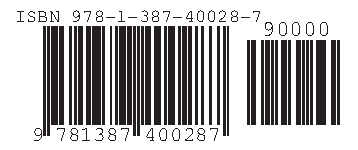
\includegraphics{isbnbarcode}

\closeout\chapterlist
\end{document}
